\documentclass[landscape,letterpaper]{seminar}
\usepackage{amsfonts}
\usepackage{fancybox}%,times}
\usepackage{graphicx,psfrag,epsf}
\usepackage{amsmath}
\usepackage{enumerate}
\newcommand{\newc}{\newcommand}

\newcommand{\bb}{\beta^{\text{bad}}}
\newcommand{\bg}{\beta^{\text{good}}}
\renewcommand{\P}{\text{P}}

% === dcolumn package ===
\usepackage{dcolumn}
\newcolumntype{.}{D{.}{.}{-1}}
\newcolumntype{d}[1]{D{.}{.}{#1}}

%\addtolength{\oddsidemargin}{-1in}
%\addtolength{\evensidemargin}{-1in}
%\addtolength{\textheight}{10in}
%\pagestyle{empty}
%\def\square{\vrule height  1.4ex width 1.3ex depth -0.1ex }

\def\dofig#1#2{\centerline{\epsfxsize=#1 \epsfbox{#2}}}
\def\dotwofig#1#2#3{\centerline{\epsfxsize=#1 \epsfbox{#2} \epsfxsize=#1
\epsfbox{#3} }}
\def\ref{\par\noindent\hangindent 10pt}

%\renewcommand{\printlandscape}{\special{landscape}}
%\slidesmag{2}
\slidesmag{3}
%\twoup

\newcommand{\heading}[1]{%
\begin{center}
\large\bf\shadowbox{#1}
\end{center}
\vspace{1ex minus 1ex}}

\begin{document}
%\slideframe{none}

%%%%%%%%%%%%%%%%%%%%%%%%%%%%%%%%%%%%%%%%%%%%%%%%%%%%%%%%%%%%%%%%%%%

\begin{slide}
\heading{Did Illegally Counted Overseas Absentee Ballots} 
\heading{Decide the 2000 US Presidential Election?}

\bigskip
\bigskip
\begin{center}
{\bf \large Kosuke Imai} \hspace{0.2in} \& \hspace{0.2in} 
{\bf \large Gary King} \\

\bigskip
Department of Government \\
Harvard University \\
\end{center}

\end{slide}

%%%%%%%%%%%%%%%%%%%%%%%%%%%%%%%%%%%%%%%%%%%%%%%%%%%%%%%%%%%%%%%%%%%

\begin{slide}
\heading{Late Overseas Absentee Ballots Determined}
\heading{the Outcome of the Election}
\bigskip

\begin{table}
\begin{center}
\begin{tabular}{lcccc}
                                 & Gore      & Bush      & margin \\ 
\hline 
Ballots cast/received by Nov.\ 7 &2,911,417 & 2,911,215 & {\bf Gore leads by 202} \\
Overseas absentee ballots        &      836 &     1,575 & Bush leads by 739 \\
\hline
Total                          & 2,912,253 & 2,912,790 & Bush leads by 537 \\
\end{tabular} \caption{Official results of the 2000 presidential
  election in Florida. \newline Source: Florida Secretary of State's office.}
\label{tb:official}
\end{center}
\end{table} 

\end{slide}

%%%%%%%%%%%%%%%%%%%%%%%%%%%%%%%%%%%%%%%%%%%%%%%%%%%%%%%%%%%%%%%%%%%

\begin{slide}
\heading{Overview}
\bigskip

\begin{itemize}
\item {\bf ILLEGALITY:} 680 of the overseas absentee ballots that had
  been counted by Florida counties \emph{unambiguously violated}
  Florida election law. In contrast, many political decisions made by
  the courts and officials were controversial but they were official,
  legal and were eventually accepted by all concerned.
\smallskip
\item {\bf POLITICAL STRATEGIES:} The illegal actions of local election
  officials were due to \emph{deliberate political strategies}
  employed by the Bush campaign.  The problem was not caused by an old
  voting machine.
\smallskip  
\item {\bf Ecological Inference with Bayesian Model Averaging:} The
  methodology is useful when substantive conclusions depend heavily on
  indefensible model choices, when model generalization is not
  feasible, and when potential critics are more partisan than
  academic.
\end{itemize}

\end{slide}

%%%%%%%%%%%%%%%%%%%%%%%%%%%%%%%%%%%%%%%%%%%%%%%%%%%%%%%%%%%%%%%%%%%

\begin{slide}
\heading{Invalid Overseas Absentee Ballots in Florida}
\bigskip

{\bf The New York Times found the following 680 illegal ballots:}

\begin{itemize}
\item 344 ballots had late, illegible or missing postmarks. \\ (postmarks
  must indicate that the ballot was cast on or before election day)
\item 183 ballots were missing United States postmarks. \\ (postmarks from
  other countries are not allowed)
\item 169 ballots were received from voters who were not registered,
  who had failed to sign the envelope, or who had not requested a
  ballot.
\item 96 ballots lacked the required signature or address of a witness
\item 19 voters cast two ballots, both of which counted.
\item 5 ballots were received after the Nov.\ 17 deadline but counted
  anyway.
\end{itemize}

\end{slide}

%%%%%%%%%%%%%%%%%%%%%%%%%%%%%%%%%%%%%%%%%%%%%%%%%%%%%%%%%%%%%%%%%%%

\begin{slide}
\heading{Ecological Inference for Flawed Ballots}

{\bf Ultimate Quantity of Interest:} Bush's margin without invalid ballots.
\smallskip
\begin{center}
\small
\begin{table}
    \begin{tabular}{ccccc}
      & Gore  & Bush & Others & total  \\
      \hline 
      invalid ballots &   ?   &   ?  &   ?    &  680   \\
      valid ballots   &   ?   &   ?  &   ?    & 1824   \\
      \hline
      & 836   & 1575 &   79   & 2504   \\
    \end{tabular} 
    \caption{\small Ecological Inference Problem in Florida.}\label{tb:ballots}
\end{table} 

\bigskip
\begin{table}
\begin{tabular}{cccc}
                & Gore  & Bush &         \\
\hline 
invalid ballots & $\bb_i$  & $1-\bb_i$ & $X_i$   \\
valid ballots   & $\bg_i$  & $1-\bg_i$ & $1-X_i$ \\
\hline
                & $T_i$ & $1-T_i$ &         \\
\end{tabular} 
\caption{\small Formulation of Ecological Estimation.}\label{tb:ei}
\end{table} 
\end{center}
\normalsize
\end{slide}

%%%%%%%%%%%%%%%%%%%%%%%%%%%%%%%%%%%%%%%%%%%%%%%%%%%%%%%%%%%%%%%%%%%

\begin{slide}
\heading{Analysis Without Statistical Assumptions}
\bigskip

{\bf Accounting Identity:} $T_i=\bb_i X_i+\bg_i (1-X_i)$.
\bigskip

{\bf Tomography line:} $\bg_i = \frac{T_i}{1-X_i}-\frac{X_i}{1-X_i}\bb_i.$

\begin{figure}
\hspace{1.4in}\begin{minipage}[l]{3in}
    \begin{center}
      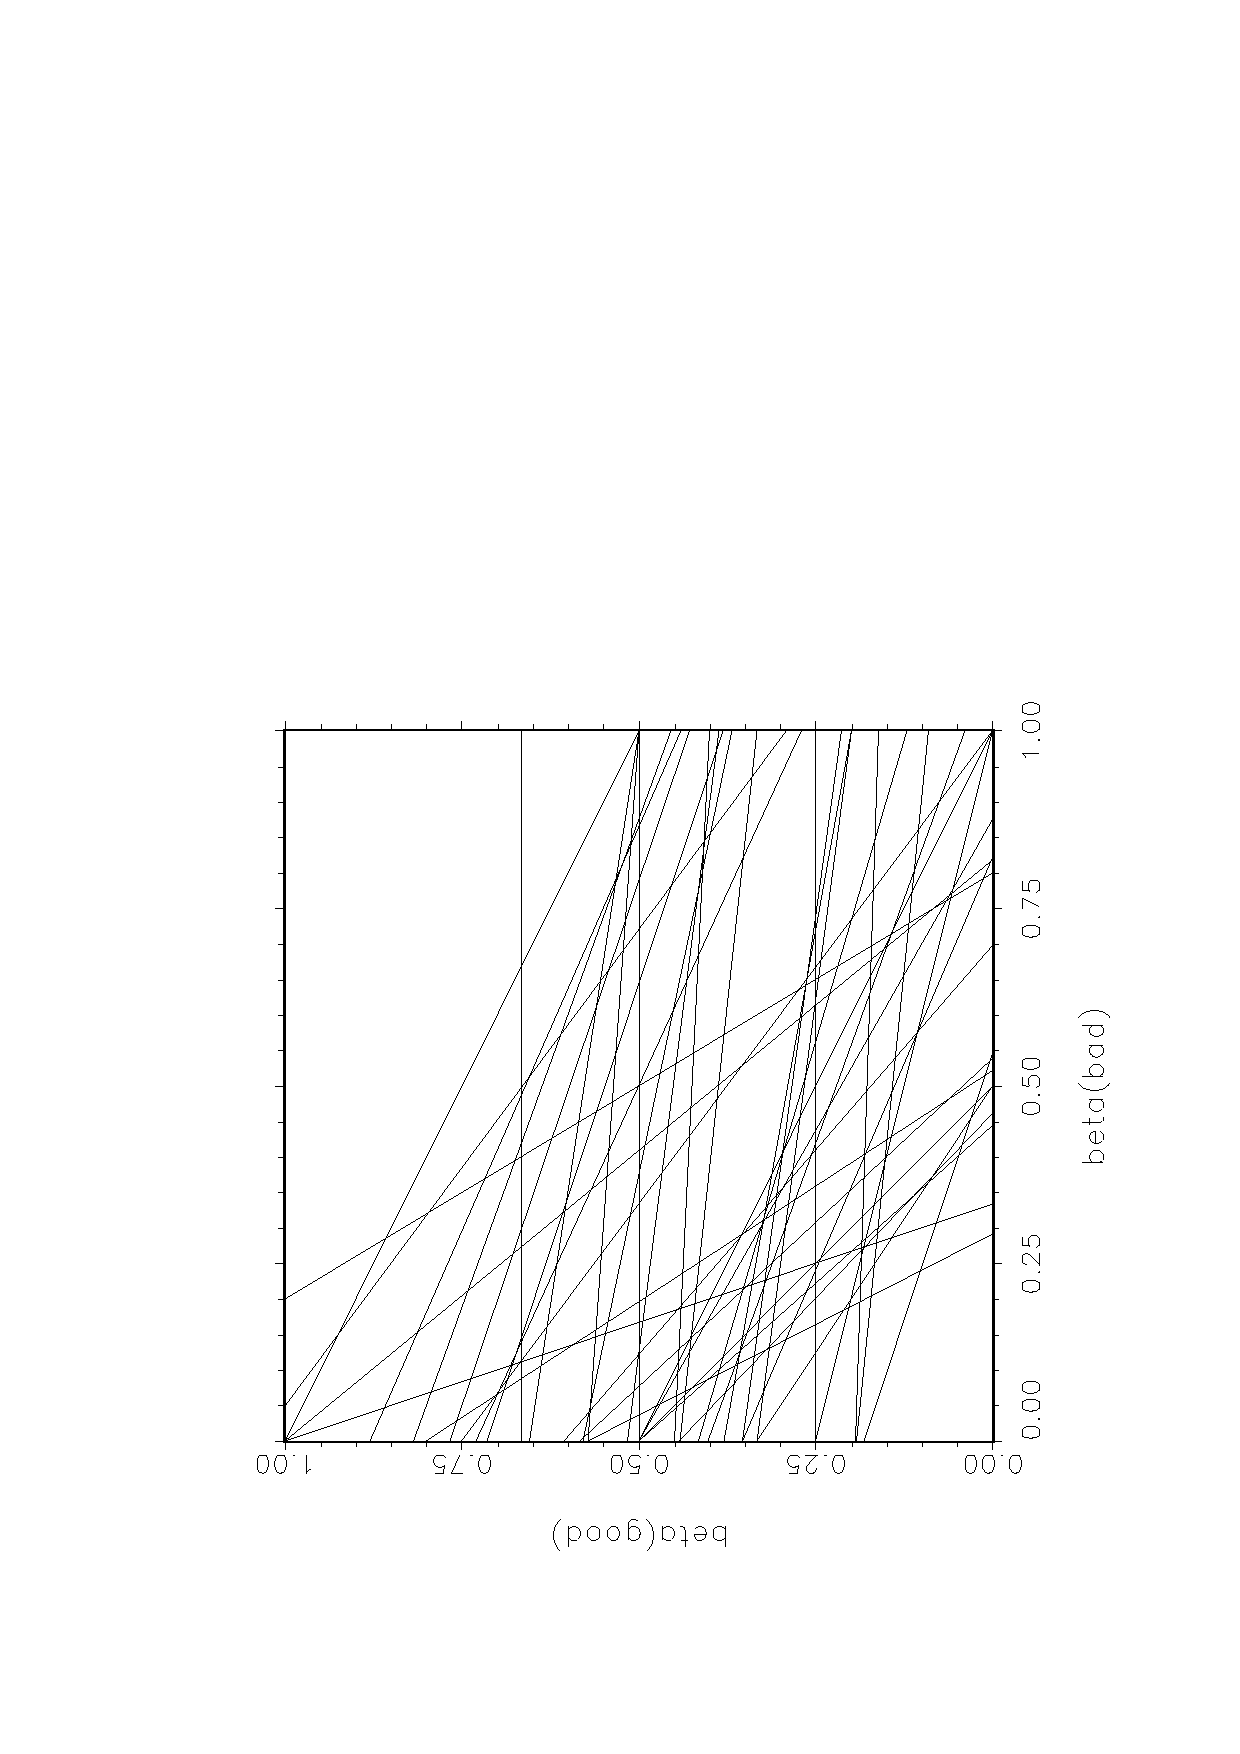
\includegraphics[width=2.25in,height=3in,angle=-90]{tomog}
    \end{center}
  \end{minipage}
  \caption{\small \label{fg:tomog} Tomography Plot for Florida Counties.}
\end{figure}

\end{slide}

%%%%%%%%%%%%%%%%%%%%%%%%%%%%%%%%%%%%%%%%%%%%%%%%%%%%%%%%%%%%%%%%%%%

\begin{slide}
\heading{Analysis of Bounds}
\bigskip

{\bf We CANNOT exclude the possibility that Gore would have won if 680
invalid ballots had not been counted.}

\smallskip
\begin{table}
\begin{center}
\begin{tabular}{l c |ccc|ccc}
  & \bf Total   & \multicolumn{3}{c|}{\bf Gore's votes} &
  \multicolumn{3}{c}{\bf Bush's votes} \\
  & invalid & official & \multicolumn{2}{c|}{invalid ballots} & official &
  \multicolumn{2}{c}{invalid ballots} \\
County & ballots & counts & min & max & counts & min & max \\
\hline 
Escambia   & 102 & 47 & 0 & 47 & 154 & 48 & 102 \\
Santa Rosa &  55 & 16 & 0 & 16 &  65 & 37 &  55 \\
Baker      &   1 &  0 & 0 &  0 &   1 &  1 &   1 \\
\hline
\bf all counties & \bf 680 & \bf 836 & \bf 5 & \bf 527 & \bf 1575 & \bf 128 & \bf 668 \\ 
\end{tabular} \caption{Analysis of bounds.}
\end{center}
\end{table} 

\end{slide}

%%%%%%%%%%%%%%%%%%%%%%%%%%%%%%%%%%%%%%%%%%%%%%%%%%%%%%%%%%%%%%%%%%%

\begin{slide}
\heading{Statistical Modeling}

{\bf Key Assumptions of King's Ecological Inference Model}
\begin{itemize}
\item The unknown parameters from Florida's 67 counties have something
  common and any systematic difference is accounted by covariates.
\item Conditional on covariates, there is no spatial correlation.
\item Conditional on covariates, $\bb_i$ and $\bg_i$ are independent
  of $X_i$. 
\end{itemize}

{\bf Difficulties of Ecological Inference}
\begin{itemize}
\item Sensitivity: Estimation results tend to be sensitive to model specification.
\item Identifiability: We cannot include many covariates in one model.
\end{itemize}

{\bf Particular Challenges of this Study}
\begin{itemize}
\item No strong theoretical guidance for model choice.
\item Need to conduct a non-partisan analysis.
\end{itemize}

\end{slide}

%%%%%%%%%%%%%%%%%%%%%%%%%%%%%%%%%%%%%%%%%%%%%%%%%%%%%%%%%%%%%%%%%%%

\begin{slide}
\heading{Bayesian Model Averaging}
\bigskip

Along with $T_i$, $X_i$ and $N_i$, we have 27 other variables
including race, sex, and party registration for the overseas absentee
voters as well as county level election and demographic data. We
define 31 different models using this data.

\smallskip

{\bf Bayesian Inference:} $\P(\Delta|T) \propto \P(\Delta)\P(T|\Delta).$

{\bf Model Averaging:} Obtain one set of results by averaging multiple
models according to the support each of them receives from the data.
\begin{align*}
  \Pr(\Delta|T) &= \sum_{k=1}^{31} \P(\Delta,M_k|T)\notag\\
                &= \sum_{k=1}^{31} \P(\Delta|M_k,T) \Pr(M_k|T).
\end{align*}
where the posterior model probability is computed as
\begin{equation*}
\Pr(M_k|T)=\frac{\P(T|M_k)\Pr(M_k)}{\sum_{j=1}^{31} \Pr(T|M_j) \Pr(M_j)}.  
\end{equation*}

\end{slide}

%%%%%%%%%%%%%%%%%%%%%%%%%%%%%%%%%%%%%%%%%%%%%%%%%%%%%%%%%%%%%%%%%%%

\begin{slide}
\heading{\small Probability that Gore Would Have Won Without Flawed Ballots}

\begin{figure}
\begin{center}
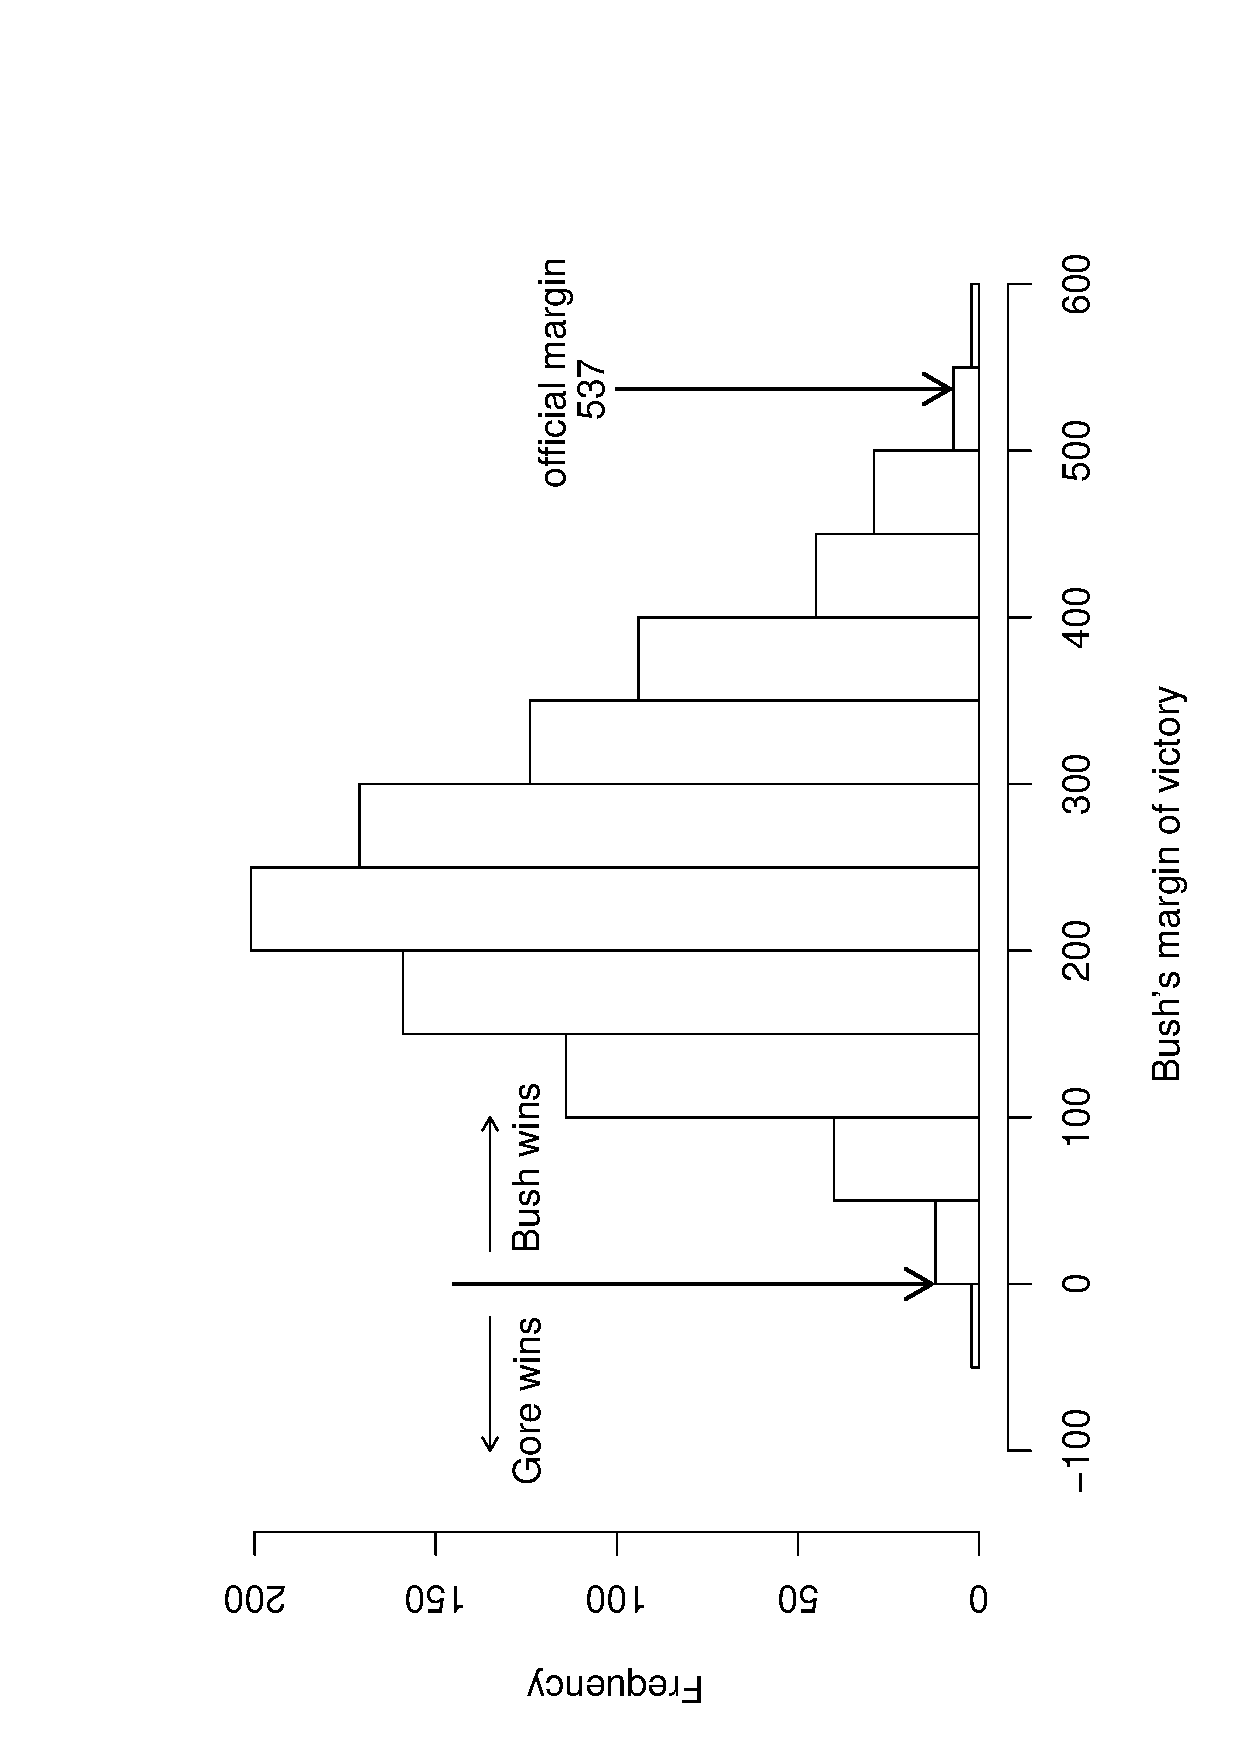
\includegraphics[width=2.5in,height=4in,angle=-90]{margin}
\caption{\small Posterior distribution of Bush's margin of victory without the
  680 invalid overseas absentee ballots} \label{fg:margin}
\end{center} 
\end{figure}
\end{slide}

%%%%%%%%%%%%%%%%%%%%%%%%%%%%%%%%%%%%%%%%%%%%%%%%%%%%%%%%%%%%%%%%%%%

\begin{slide}
\heading{Other Counterfactuals}

\begin{table}
\small
\begin{center}
\begin{tabular}{l..}
 & \multicolumn{1}{c}{Bush's margin} & \multicolumn{1}{c}{Prob(Gore Wins)}\\
\hline
Invalid overseas ballots alone & 251  & 0.002 \\
\emph{Actual recounts}\\
\hspace{1em} Miami Dade partial recount     &  94  & 0.19 \\
\hspace{1em} Palm Beach recount             &  59  & 0.29 \\
\hspace{1em} Miami Dade and Palm Beach    & -98  & 0.82 \\
\emph{Media recounts}\\
\hspace{1em} No U.S.\ Supreme Court decision  & 242  & 0.01\\
\hspace{1em} Gore's request granted         & -26  & 0.73\\
\hspace{1em} only fully punched ballots     & -366 & >0.99 \\
\hspace{1em} hanging chads and dimples      & -358 & >0.99 \\
\hspace{1em} each county's standard         & -422 & >0.99 \\
\end{tabular}
\end{center}
\caption{\small Estimated margin and probability of victory with selected
counterfactuals} \label{tb:senario}
\end{table}
\normalsize
\end{slide}

%%%%%%%%%%%%%%%%%%%%%%%%%%%%%%%%%%%%%%%%%%%%%%%%%%%%%%%%%%%%%%%%%%%

\begin{slide}
\heading{Indirect Evidence of Local Election Officials} 
\heading{Responding to Republican Pressure}
\bigskip

\begin{itemize}
\item The \emph{New York Times} concluded ``Their [Republicans'] goal was
simple: to count the maximum number of overseas ballots in counties
won by Mr.  Bush, particularly those with a high concentration of
military voters, while seeking to disqualify overseas ballots in
counties won by Vice President Al Gore.''

\bigskip
\item The \emph{Times} claimed that as a direct result of this pressure,
``canvassing boards in about a dozen Republican-leaning counties had
reconvened for a second round of counting.  In each place,
longstanding election rules were bent and even ignored.  Boards
counted ballots postmarked as many as seven days after the election,
including some from within the United States.  They counted two
ballots sent by fax.  Officials in Santa Rosa County even counted five
ballots that arrived after the Nov.\ 17 deadline.  Again and again,
election officials crossed out the words `REJECTED AS ILLEGAL' that
had been stamped on ballot envelopes.''
\end{itemize}
  
\end{slide}

%%%%%%%%%%%%%%%%%%%%%%%%%%%%%%%%%%%%%%%%%%%%%%%%%%%%%%%%%%%%%%%%%%%

\begin{slide}
\begin{table}
\footnotesize
\begin{tabular}{l....|.}
& \multicolumn{1}{c}{military} 
& \multicolumn{1}{c}{Republican} 
& \multicolumn{1}{c}{Bad ballot}
& \multicolumn{1}{c}{Bad Ballots} 
\\ 
& \multicolumn{1}{c}{ballots} 
& \multicolumn{1}{c}{vote} 
& \multicolumn{1}{c}{acceptance}
& \multicolumn{1}{c}{counted for Bush} 
& \multicolumn{1}{c}{all ballots}\\    \hline
    \multicolumn{4}{l}{\bf Republican pressure to count} \\
    \hspace{1em}Collier  & 46.7\% & 65.6\% & 53.7\% & 64.5\% & 60 \\    
    \hspace{1em}Duval    & 83.8 & 57.5 & 62.3 & 67.8 & 637 \\
    \hspace{1em}Escambia & 88.6 & 62.6 & 64.2 & 80.3 & 272 \\         
    \hspace{1em}Okaloosa & 88.9 & 73.7 & 42.0 & 69.4 & 189 \\          
    \hspace{1em}Pasco    & 62.3 & 48.0 & 60.5 & 76.4 & 53 \\                
    \hspace{1em}Santa Rosa & 90.3 & 72.1 & 84.6 & 84.4 & 93 \\
    \hspace{1em}\emph{Average} & \emph{83}.\emph{4} & \emph{60}.\emph{0} & \emph{61}.\emph{5} & \emph{74}.\emph{3} & 1304 \\
\multicolumn{5}{l}{\bf Counties not mentioned by the \emph{Times}}
& \\ 
\hspace{1em}\emph{Average} & \emph{67}.\emph{6} & \emph{51}.\emph{8} & \emph{30}.\emph{0} & \emph{71}.\emph{5} & 1751\\
\multicolumn{4}{l}{\bf Republican pressure not to count}\\ 
    \hspace{1em}Alachua    & 46.8 & 39.8 & 12.5 & 54.5 & 77 \\ 
    \hspace{1em}Broward    & 46.9 & 30.9 & 21.8 & 54.3 & 213 \\  
    \hspace{1em}Miami Dade & 44.4 & 46.3 & 11.7 & 57.1 & 306 \\
    \hspace{1em}Palm Beach & 45.3 & 35.3 & 40.7 & 56.2 & 53 \\ 
    \hspace{1em}\emph{Average} & \emph{45}.\emph{6} & \emph{38}.\emph{1} & \emph{17}.\emph{2} & \emph{55}.\emph{4} &  649 \\
    \hline                                                       
  \end{tabular}                                                
  \caption{\footnotesize Counties classified by whether the \emph{Times} reported evidence of Republican pressure.} 
\end{table}

\end{slide}

%%%%%%%%%%%%%%%%%%%%%%%%%%%%%%%%%%%%%%%%%%%%%%%%%%%%%%%%%%%%%%%%%%%

\begin{slide}
\heading{Qualitative Evidence Backs Up Statistical Analysis}
\bigskip

\begin{itemize}
\item The \emph{Times} reported that an election official on the Duval
  County canvassing board ``held the line on counting ballots with
  missing postmarks.''

\bigskip
  
\item the story also described the unusually strong Republican
  pressure applied in \emph{Pasco county}: ```It looks to me like
  we've got a lot of pressure here,' Judge Robert P.  Cole, chairman
  of the Pasco board, said as he faced a throng of cheering
  Republicans and more than a dozen Bush representatives [and no
  officials from the Gore campaign].''
\end{itemize}

\end{slide}

%%%%%%%%%%%%%%%%%%%%%%%%%%%%%%%%%%%%%%%%%%%%%%%%%%%%%%%%%%%%%%%%%%%

\begin{slide}
\heading{Results of Bayesian Model Averaging}
\small
\begin{table}
\begin{center}
\begin{tabular}{l c r@{, }l d{3} d{-3}}
  & \multicolumn{3}{c}{Bush's margin}& \multicolumn{1}{c}{first} 
  & \multicolumn{1}{c}{Posterior model} \\
  & \multicolumn{3}{c}{(95 \% C.I.)} & \multicolumn{1}{c}{difference} 
  & \multicolumn{1}{c}{probability} \\
\hline
\multicolumn{1}{l}{Bayesian Model Averaging} & 251 & (69 & 468) & \\
\multicolumn{1}{l}{\emph{Individual models}}  \\ 
\hspace{0.5em} Registered Repub.\ absentee voters
 & 269 & (97 & 475) & $-52$ &  0.565 \\
\hspace{0.5em} Dem.\ vote share
 & 232 & (69 & 448) & 3 &  0.239 \\
\hspace{0.5em} Black absentee voters
 & 231 & (69 & 440) & $-2$ &  0.102 \\
\hspace{0.5em} White absentee voters
 & 123 & ($-$18& 315) & $-23$ &  0.033 \\
\hspace{0.5em} Registered black Repubs
 & 229 & (62 & 441) & $-6$ &  0.021 \\
\hspace{0.5em} Accepted absentee ballots
 & 218 & (62 & 409) & 4 &  0.004 \\
\end{tabular}
\caption{Estimates of Bush's margin of victory after dropping the
  invalid overseas absentee ballots.}
\label{tb:bma}
\end{center}
\end{table}

\end{slide}

%%%%%%%%%%%%%%%%%%%%%%%%%%%%%%%%%%%%%%%%%%%%%%%%%%%%%%%%%%%%%%%%%%%

\begin{slide}
\heading{Model Fit}

\begin{figure}
\hspace{0.5in}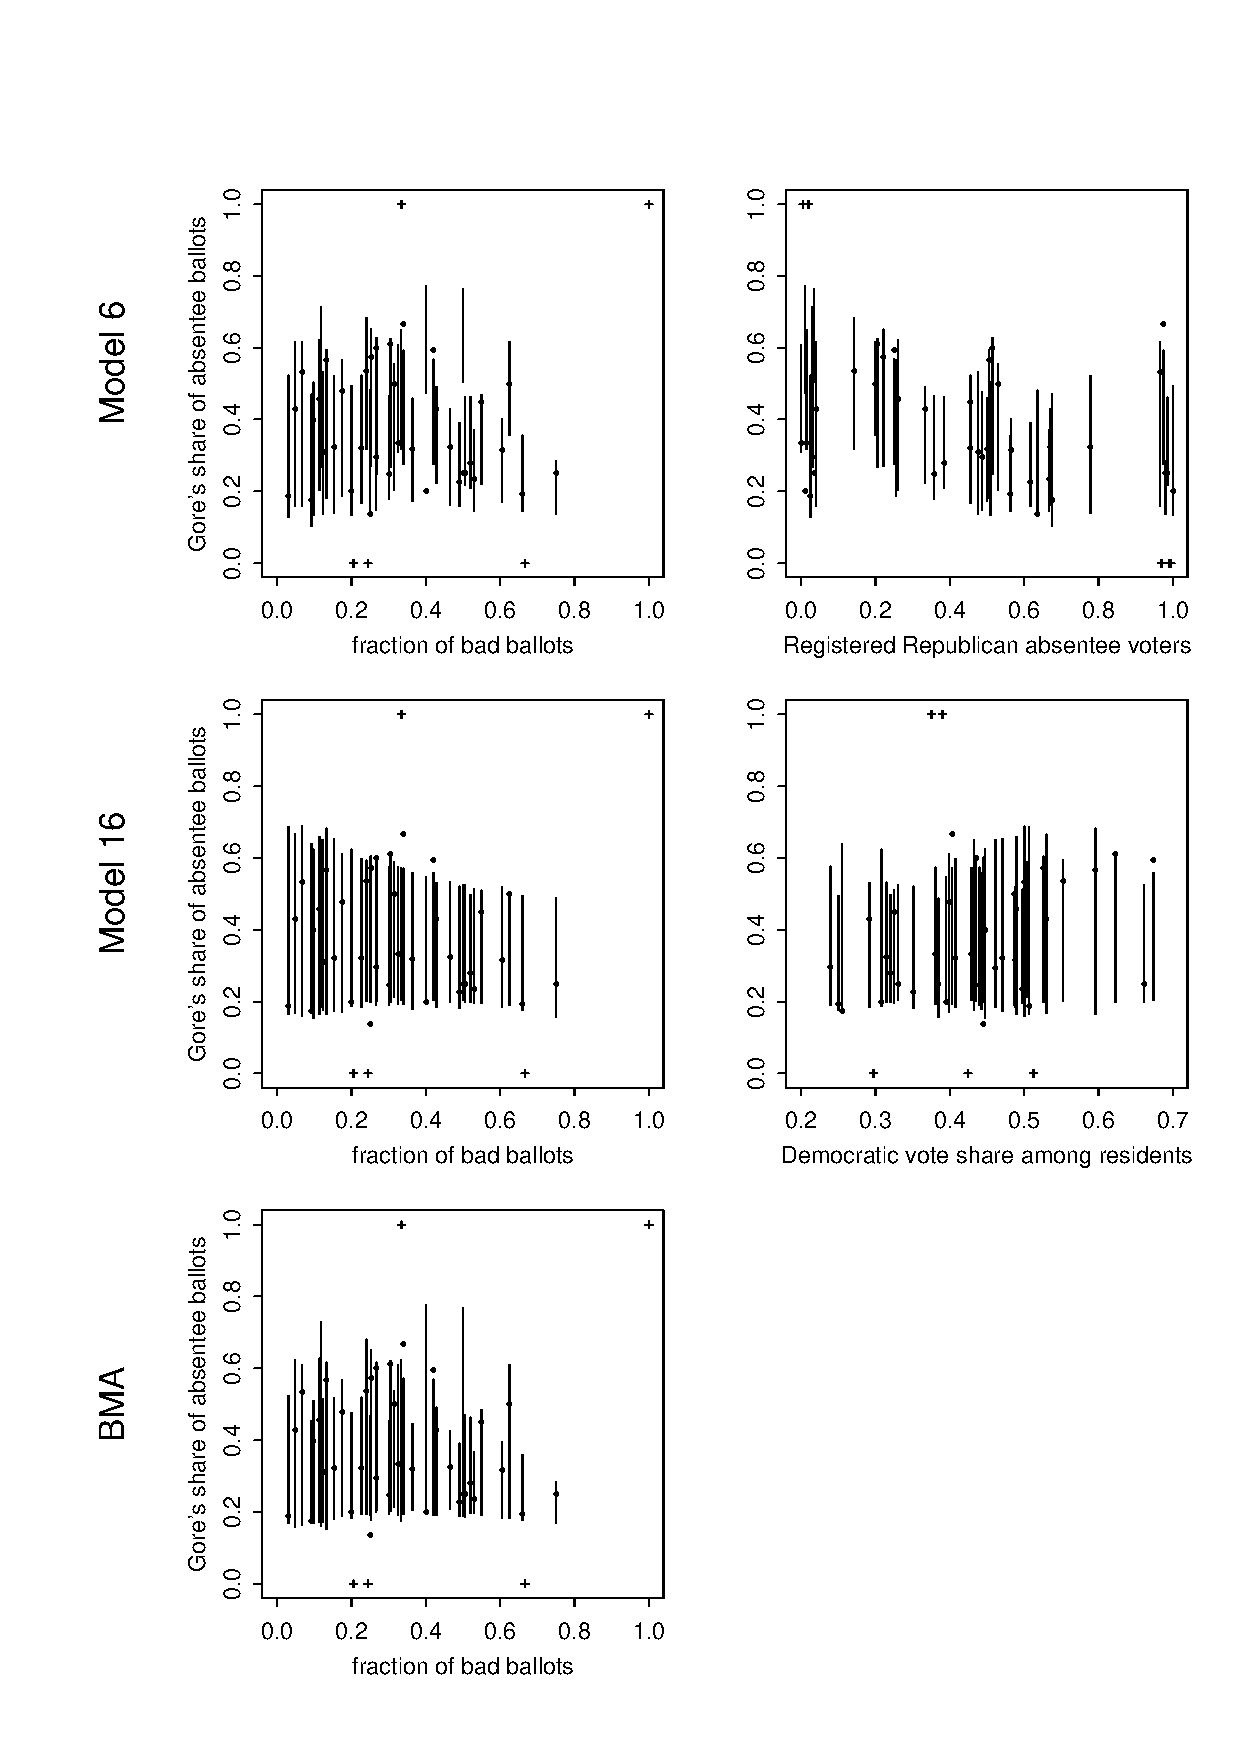
\includegraphics[width=4in,height=3in]{fit}
\caption{\small Posterior predicted distribution of $T_i$, (80\%
  confidence intervals).}
\end{figure}
\end{slide}

%%%%%%%%%%%%%%%%%%%%%%%%%%%%%%%%%%%%%%%%%%%%%%%%%%%%%%%%%%%%%%%%%%%

\begin{slide}
\heading{Sensitivity Analysis}
\begin{figure}
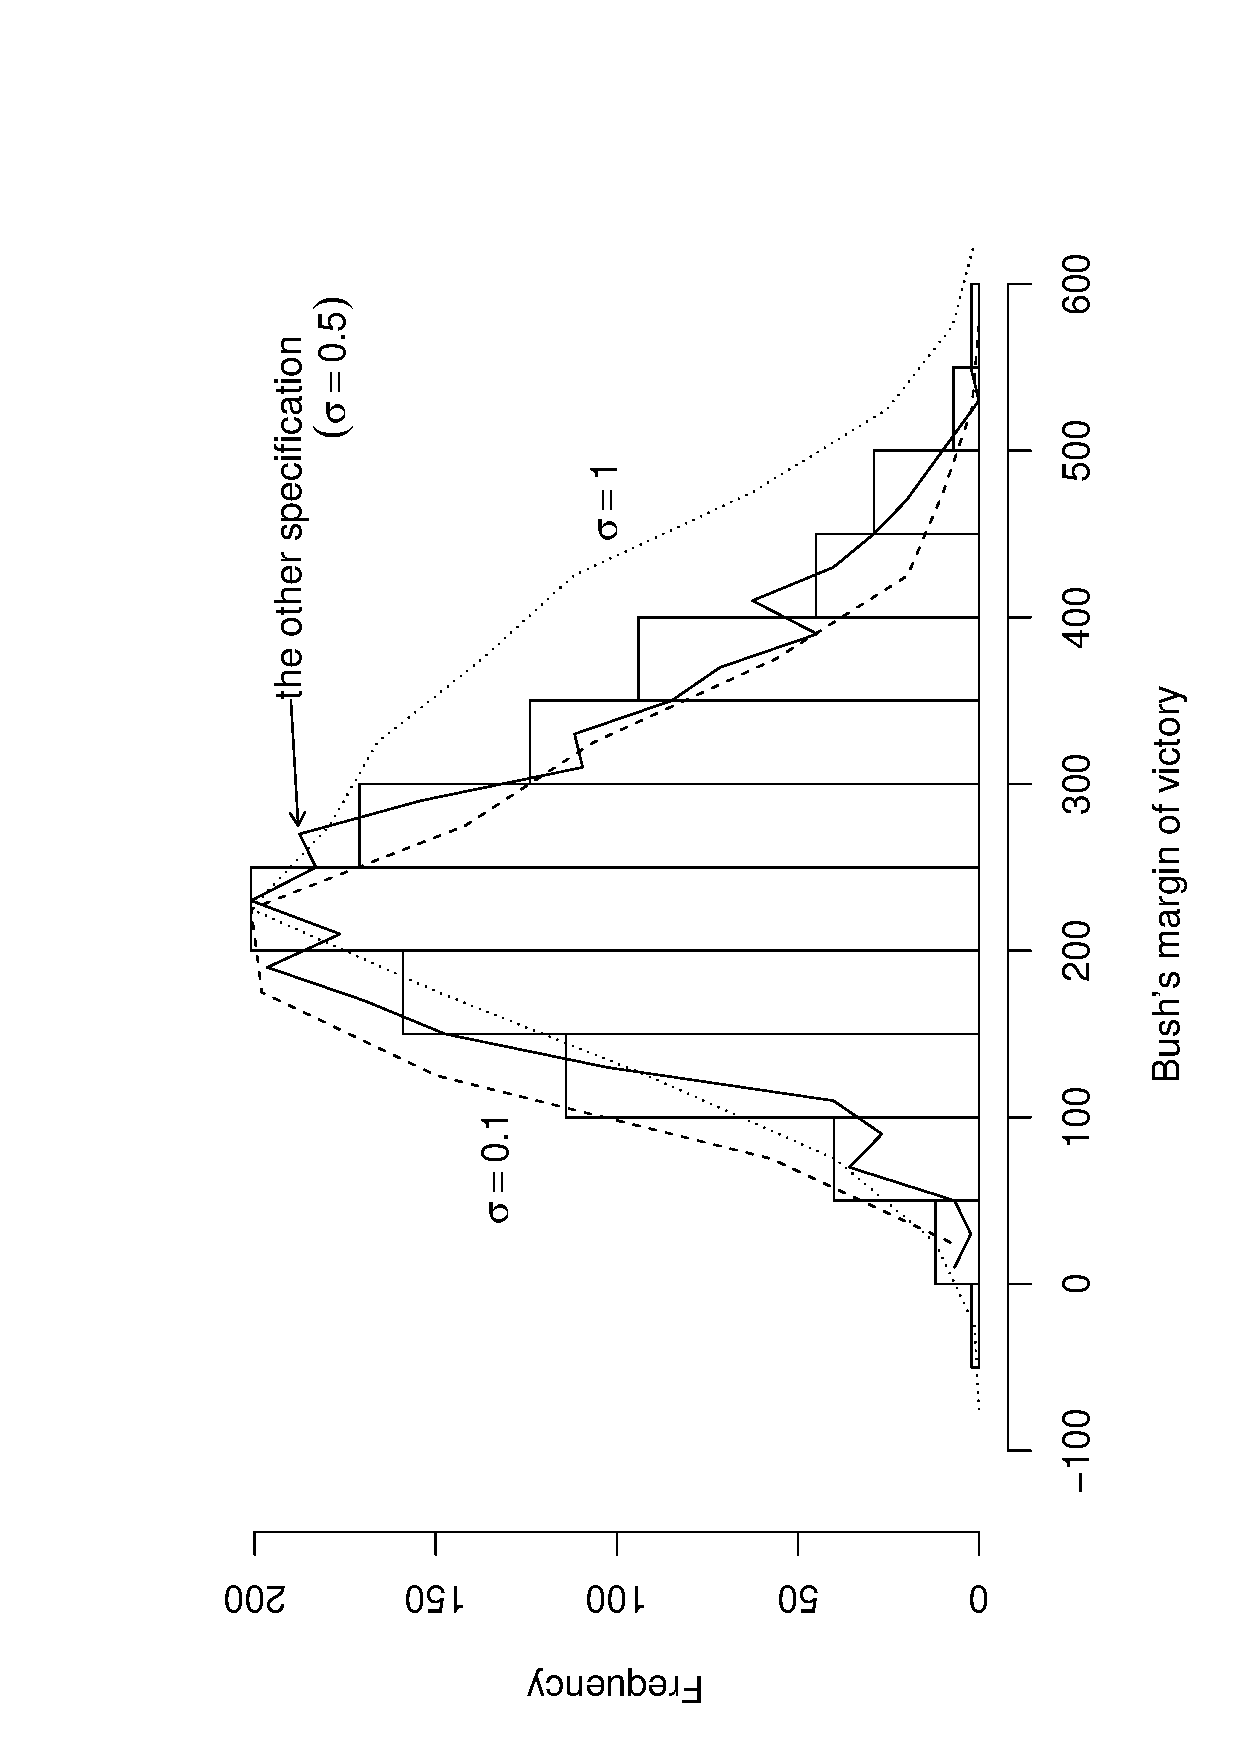
\includegraphics[width=3in,height=4.5in,angle=-90]{sensitivity}
\caption{\small Sensitivity analysis of Bayesian model averaging.}
\end{figure}
\end{slide}

%%%%%%%%%%%%%%%%%%%%%%%%%%%%%%%%%%%%%%%%%%%%%%%%%%%%%%%%%%%%%%%%%%%

\begin{slide}
\heading{Concluding Remarks}
\bigskip

\begin{itemize}
\item {\bf Bush won? But we will never know with certainty:} Some
  scenarios show the high probability that Gore would have won.

\item {\bf Strong support for the \emph{New York Times} thesis:}
  Quantitative evidence confirms qualitative stories.

\item {\bf Validity of counterfactuals:} When the counterfactual is
  very close to the data, we stand an especially good chance of making
  valid inference. The counterfactual questions we ask in this paper
  represent such a situation.

\item {\bf First application of Bayesian model averaging in Political
    Science:}  A clear improvement on the usual situation of having to
  select and defend a single model. A contribution to Ecological
  Inference literature. However, model averaging cannot substitute for
  the investigator's judgment.

\end{itemize}

\end{slide}

\end{document}


